\hypertarget{time-to-close}{%
\subsubsection{Time to Close}\label{time-to-close}}

Question: How much time passes between creating and closing an operation
such as an issue, change request, or support ticket?

\hypertarget{description}{%
\paragraph{Description}\label{description}}

The time to close is the total amount of time that passes between the
creation and closing of an operation such as an issue, change request,
or support ticket. The operation needs to have an open and closed state,
as is often the case in code review processes, question and answer
forums, and ticketing systems.

Related metric:
\href{https://chaoss.community/metric-issue-resolution-duration/}{Issue
Resolution Duration}

\hypertarget{objectives}{%
\paragraph{Objectives}\label{objectives}}

\begin{enumerate}
\def\labelenumi{\arabic{enumi}.}
\tightlist
\item
  Determining how responsive a community is can help efforts to be
  inclusive, attract, and retain new and existing contributors.
\item
  Identifying characteristics of operations that impact an operation
  closing quickly or slowly (e.g., finding best practices, areas of
  improvement, assess efficiency).
\item
  Identifying bias for timely responses to different community members.
\item
  Detecting a change in community activity (e.g., to indicate potential
  maintainer burnout, reduction in the diversity of contributions)
\item
  Understand how the time to close an issue or change request is related
  to merge success or failure.
\end{enumerate}

\hypertarget{implementation}{%
\paragraph{Implementation}\label{implementation}}

\hypertarget{filters}{%
\subparagraph{Filters}\label{filters}}

\begin{itemize}
\tightlist
\item
  Creator of operation (e.g., new contributor vs. maintainer)
\item
  First closed, final closed
\item
  Labels (e.g., bug vs. new feature)
\item
  Change Request Merge Status (e.g. Time to Merge or Time to Close
  without Merge)
\end{itemize}

\hypertarget{visualizations}{%
\subparagraph{Visualizations}\label{visualizations}}

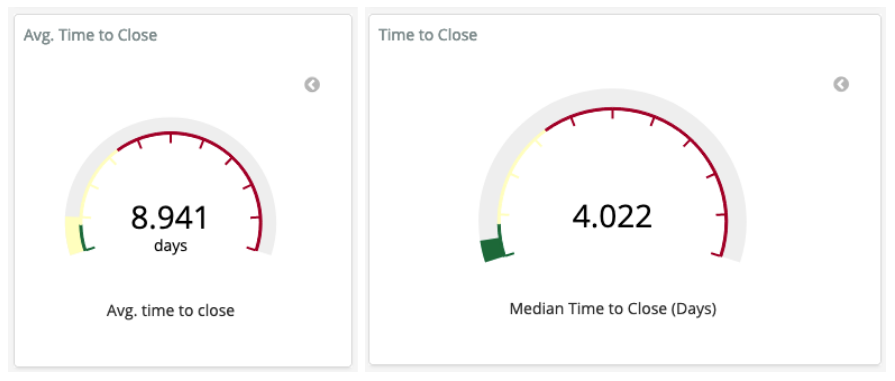
\includegraphics{images/time-to-close_1.png}

\hypertarget{tools-providing-the-metric}{%
\subparagraph{Tools Providing the
Metric}\label{tools-providing-the-metric}}

Augur implementation:

\begin{itemize}
\tightlist
\item
  \href{http://augur.osshealth.io/api_docs/\#api-Evolution-Closed_Issue_Resolution_Duration(Repo)}{Issue
  Close Duration}
\item
  \href{http://augur.osshealth.io/api_docs/\#api-Evolution-issue-duration-repo}{Issue
  Duration}
\item
  \href{http://augur.osshealth.io/api_docs/\#api-Evolution-Issue_Response_Time(Repo)}{Issue
  Response Time}
\end{itemize}

GrimoireLab implementation:

\begin{itemize}
\tightlist
\item
  \href{https://chaoss.github.io/grimoirelab-sigils/panels/github-pullrequests-efficiency/}{Pull
  Requests Efficiency}
\item
  \href{https://chaoss.github.io/grimoirelab-sigils/panels/github-issues-efficiency/}{Issues
  Efficiency}
\item
  \href{https://chaoss.github.io/grimoirelab-sigils/panels/efficiency-timing-overview/}{Efficiency:TimingOverview}
\end{itemize}

\hypertarget{data-collection-strategies}{%
\subparagraph{Data Collection
Strategies}\label{data-collection-strategies}}

The time to close metric may be contextual based on the project activity
and objectives. For example, the time to close a bug report may provide
different information than the time to close a new feature request. Data
collection strategies should address different project objectives. Other
variables that may influence these processes are:

\begin{itemize}
\tightlist
\item
  Issue Tracking Systems: the type of issue such as bug report,
  blueprint (OpenStack nomenclature), user story, feature request, epic,
  and others may influence how long this event takes to be closed. Other
  variables, such as the priority or severity may help to advance how
  quickly this event will be closed.
\item
  Change Request Processes: this depends on the change request
  infrastructure, as Gerrit, GitHub or mailing lists (as in the Linux
  Kernel) and may differ depending on how complicated the process is.
  For example, newcomers or advanced and experienced developers will
  proceed in different ways and with more or less time required.
\item
  Question and Answer Forum: this depends on the quality of the answer
  and the opinion of the person asking the question. A valid answer is
  marked, and the process is closed once the person questioning has
  successfully found a correct answer to their question.
\end{itemize}

\hypertarget{references}{%
\paragraph{References}\label{references}}

\begin{itemize}
\tightlist
\item
  ``Practice P.12: Respond to all submissions'' from ``Appendix to:
  Managing Episodic Volunteers in Free/Libre/Open Source Software
  Communities'' by Ann Barcomb, Klaas-Jan Stol, Brian Fitzgerald and
  Dirk Riehle:
  \href{https://opus4.kobv.de/opus4-fau/frontdoor/index/index/docId/13519}{https://opus4.kobv.de/opus4-fau/frontdoor/index/index/docId/13519}
\end{itemize}
